%
% File acl2020.tex
%
%% Based on the style files for ACL 2020, which were
%% Based on the style files for ACL 2018, NAACL 2018/19, which were
%% Based on the style files for ACL-2015, with some improvements
%%  taken from the NAACL-2016 style
%% Based on the style files for ACL-2014, which were, in turn,
%% based on ACL-2013, ACL-2012, ACL-2011, ACL-2010, ACL-IJCNLP-2009,
%% EACL-2009, IJCNLP-2008...
%% Based on the style files for EACL 2006 by 
%%e.agirre@ehu.es or Sergi.Balari@uab.es
%% and that of ACL 08 by Joakim Nivre and Noah Smith

\documentclass[11pt,a4paper]{article}
\usepackage[hyperref]{acl2020}
\usepackage{times}
\usepackage{latexsym}
\renewcommand{\UrlFont}{\ttfamily\small}
\usepackage{booktabs}
\usepackage{multirow}
\usepackage{tikz}
\usepackage{amsmath}
\usepackage{graphicx}
\usepackage{natbib}
% This is not strictly necessary, and may be commented out,
% but it will improve the layout of the manuscript,
% and will typically save some space.
\usepackage{microtype}

\usepackage{tabularx}
\newcolumntype{L}{>{\raggedright\arraybackslash}X}

%\aclfinalcopy % Uncomment this line for the final submission
%\def\aclpaperid{***} %  Enter the acl Paper ID here

%\setlength\titlebox{5cm}
% You can expand the titlebox if you need extra space
% to show all the authors. Please do not make the titlebox
% smaller than 5cm (the original size); we will check this
% in the camera-ready version and ask you to change it back.

\newcommand\BibTeX{B\textsc{ib}\TeX}

\title{Pre-trained encoders for dialogue: The case of laughter}

\author{First Author \\
  Affiliation / Address line 1 \\
  Affiliation / Address line 2 \\
  Affiliation / Address line 3 \\
  \texttt{email@domain} \\\And
  Second Author \\
  Affiliation / Address line 1 \\
  Affiliation / Address line 2 \\
  Affiliation / Address line 3 \\
  \texttt{email@domain} \\}

\date{}

\begin{document}
\maketitle
\begin{abstract}
  In this paper, we investigate the usefulness of BERT for dialogue act recognition.
  We are interested in both how useful the pre-training procedure is and 
  how well the model adapts to the dialogue domain.
  To confirm that the fine-tuned model learns to represent dialogical features, 
  we look at how it uses laughter, a phenomenon specific to dialogue.
\end{abstract}

% INTRODUCTION

Recently, large-scale language models, trained on massive corpora of text data, have achieved state-of-the-art results on a variety of traditional NLP tasks.
It is still uncertain whether these models might be useful for processing dialogue, and if so, whether they can adapt to make use of dialogue-specific features.

Dialogue, especially spoken dialogue, is radically different from the kind of data that neural language models are pre-trained on.
In the example from the Switchboard corpus, shown in Table~\ref{table:example}, it is evident that the syntactic structure of dialogue is very different from  written text, even if one imagines a script for a movie or a play.
Not only is the internal structure of contributions different---with features such as disfluencies, repair, incomplete sentences, and various vocal sounds---but the sequential structure of the discourse is also very different.
In dialogue, speakers take turns and switch perspectives.
More generally, the way that utterances contribute to and cohere with the discourse is different from the relationship between sentences in a piece of written text.

One important dialogical feature missing from text data is laughter, which is ubiquitous in our everyday interactions.
We observe that in the Switchboard dialogue corpus laughter comes about every 200 tokens.
Laughter also relates to the discourse structure of dialogue and can relate to a laughable, which can be any an event or an entity in the discourse (and external perceived event as well).
Laughter can precede, follow or overlap the laughable, with the time alignment between the laughter and laughable dependent on who produces the laughable and the form of the laughter \citep{tian2016we}.
Laughter can act as a contextual feature for determining the sincerity of an utterance, in order to understand sincerity of an utterance, e.g. to detect sarcasm \citep{tepperman2006yeah}.

\begin{table}
      \small
  \centering
  \begin{tabularx}{\linewidth}{llL}
    \toprule
    Speaker & DA & Utterance \\ \midrule
    A	&sd	& Well, I'm the kind of cook that I don't normally measure things,  \\
    A	&sd	& I just kind of throw them in \\
    A	&sd	& and, you know, I don't to the point of, you know, measuring down to the exact amount that they say.  \\
    B	&sv	& That means you're a real cook. \\
    A	&bd	& \texttt{<Laughter>} Oh, is that what it means.  \\
    A	&b	& Uh-huh.  \\
    A	&x	& \texttt{<Laughter>}.\\
             \bottomrule
  \end{tabularx}
  \caption{Example from the SWDA corpus (sw2827). Dialogue acts: \emph{sd}---Statement-non-opinion, \emph{sv}---Statement-opinion, \emph{bd}---Downplayer, \emph{b}---Backchannel, \emph{x}---Non-verbal. }
  \label{table:example}
\end{table}

We use dialogue act recognition (DAR) as a proxy task, since both the internal content of contributions, and their sequential structure have bearing on this task. DAR is the task of assigning a dialogue act to every utterance in the dialogue, according to dialogue act that they perform.
This is the way to investigate whether transfer learning techniques based on pre-trained language models, such as BERT \citep{devlinBERTPretrainingDeep2018}, are useful for dialogue.
We looked at laughter that is certainly missing in pre-trained model, and discovered that it can be useful to disambiguate a dialogue act.

\paragraph{Contributions}
The main results of this paper have to do with to the usefulness of language model fine-tuning for DAR, the impact of laughter on DAR, and the relationship between the two.
\begin{itemize}
  \item Laughter is useful for dialogue act recognition, and its impact varies across different dialogue acts (\S\ref{sec:experiment1}).
  \item During fine-tuning, BERT learns to represent laughter, a dialogical feature not seen in pre-training (\S\ref{sec:experiment1} and \S\ref{sec:experiment2}).
  \item Standard BERT pre-training is useful for DAR, but the model performs poorly without fine-tuning (\S\ref{sec:experiment2})
  \item Further pre-training with in-domain data shows promise for dialogue (\S\ref{sec:experiment3}), but further investigation with larger dialogue corpora is required.
  \end{itemize}

In the following section we provide more details about the dialogue act recognition task and transfer learning techniques. 


\section{Background}

\subsection{Dialogue Act Recognition}
The concept of a dialogue act is based on that of speech acts \citep{austinHowThingsWords2009}.
Breaking with classical semantic theory, speech act theory considers not only the propositional content of an utterance but also the actions, such as \emph{promising} or \emph{apologizing}, it carries out.
Dialogue acts extend the concept of the speech act, with a focus on the interactional nature of most speech.
DAMSL \citep{coreCodingDialogsDAMSL1997}, for example, is an influential dialogue act tagging scheme where dialogue acts are defined in part by whether they have a \emph{forward-looking} function (are expecting a response) or \emph{backward-looking} function (are in response to a previous utterance).

DAR is the task of labeling utterances with the dialogue act they perform from a given set of dialogue act tags.
As with other sequence labeling tasks in NLP, some notion of context is helpful in DAR.
One of the first performant machine learning models for DAR was a Hidden Markov Model that used various lexical and prosodic features as input \citep{stolckeDialogueActModeling2000}.

Most successful neural approaches also model some notion of context.
We follow previous work that models dialogue act sequences with an RNN over utterances \citep{kalchbrennerRecurrentConvolutionalNeural2013,tranHierarchicalNeuralModel2017,botheContextbasedApproachDialogue2018}.
Our model predicts the most likely tag given the hidden state of the RNN at each position, though other work has shown that DAR benefits from more sophistacted approaches, such as conditional random field \citep{chenDialogueActRecognition2017} or uncertainty propegation \citep{tranPreservingDistributionalInformation2017}. 

\subsection{Transfer learning for NLP}
Transfer learning techniques allow a model trained on one task---often unsupervised---to be applied to another. 
Since annotating natural language data is expensive, there is a lot of interest in transfer learning for natural language processing. 
Word vectors \citep[e.g.,][]{mikolovDistributedRepresentationsWords2013,penningtonGloveGlobalVectors2014} are a ubiquitous example of transfer learning in NLP.
We note, however, that pre-trained word vectors are not always useful when applied to dialogue domains \citet{cerisaraEffectsUsingWord2vec2017}. 

Recently, neural models trained on large datasets with various unsupervised tasks have found success creating sentence-level and contextual word representations. 
BERT, a multi-layer tranformer, is one such model \citep{devlinBERTPretrainingDeep2018} . 
BERT is pre-trained on two unsupervised tasks: \emph{masked token prediction} and \emph{next sentence prediction}.
In masked token prediction, some percentage of words are randomly replaced with a \texttt{[MASK]} token, and the model is trained to predict the identity of these tokes based on the context sentence.
In next sentence prediction, the model is give two sentences and trained to predict whether the second sentence follows the first in the original text, or if it was randomly chosen from elsewhere in the corpus.
After pre-training, BERT can be applied to a supervised task by adding additional un-trained layers that take the hidden state of one or more of BERT's layers as input. 

There is some preivous work applying BERT to dialogue.
\citet{baoPLATOPretrainedDialogue2019,chenSemanticallyConditionedDialog2019a} and both use BERT for dialogue generation tasks.
Similarly \citet{vigComparisonTransferLearningApproaches2019} finds BERT useful for selecting a response from a list of candidate responses in a dialogue.
Finally, \citet{mehriPretrainingMethodsDialog2019} evaluates BERT in various dialogue tasks including DAR, and find that a model incorporating BERT outperforms a baseline model.

\paragraph{Fine-tuning vs.~further in-domain pre-training}
Transfer learning schemes for pre-trained language models such as BERT draw on one or more of the following three adaptation strategies \citet{sunHowFineTuneBERT2019}:
\emph{further pre-training}, in which the model is trained in an un-supervised way, similar to its initial training scheme, but on data that is in-domain for the target task; 
\emph{single-task fine-tuning}, in which the model's encoder layers are optimized during training for the target task;
and \emph{multi-task fine-tuning}, in which models with shared encoder layers are jointly trained on several related tasks.
In this paper, we investigate the first two methods and their combination, as applied to DAR.

Regardless of whether an encoder model has undergone further in-domain pre-training, the choice of whether to fine-tune during task training remains.
Freezing the encoder model during task training is more efficient, since the gradient of the loss function need only be computed for the task-specific layers.
However, fine-tuning can lead to better performance since the encoding itself is adapted to the target task and domain.

\citet{petersTuneNotTune2019} investigate when and whether to fine-tune BERT for sentence classification tasks.
They find that when the target task is very similar to the pre-training task, fine-tuning provides less of a performance boost.
There is some conceptual relationship between DAR and next sentence prediction, since the a dialogue act constrains (or at least is predictive of) the dialogue act that follows it.

\citet{petersTuneNotTune2019} also consider whether the similarity of the pre-training and target domains may have similar consequences, but don't find an effect of domain similarly for the natural language inference tasks they tested on.
As discussed in \S\ref{sec:data}, however, there are dramatic differences between written text and transcribed dialogue which may mean that fine-tuning is necessary in this case.


\section{Data}\label{sec:data}
We perform experiments on the Switchboard Dialogue Act Corpus (SWDA), which is a subset of the larger Switchboard corpus, and the dialogue act-tagged portion of the AMI Meeting Corpus (AMI-DA). 
SWDA is tagged with a set of 220 dialogue act tags which, following  \citet{jurafskySwitchboardSWBDDAMSLShallowDiscourseFunction1997a} we cluster into a smaller set of 42 tags.
AMI uses a smaller tagset of 16 dialogue acts \citep{GuidelinesDialogueAct2005}.

% - DA distribution              % Vlad

\begin{table}[]
\centering
\begin{tabular}{@{}ll@{}}
\toprule
\textbf{Switchboard}       & \textbf{AMI Corpus}                     \\ \midrule
Dyadic                     & Multi-party                             \\
Casual conversation        & Mock business meeting                   \\
Telephone                  & In-person \& video                      \\ \midrule
English                    & English                                 \\ 
Native speakers            & Native \& non-native speakers           \\ 
early '90s                 & 2000s                                   \\ \midrule
2200 conversations         & 171 meetings                            \\
  \hspace{1em} 1155 in SWDA               & \hspace{1em} 139 in AMI-DA                           \\
400k utterances             & 118k utterances                         \\
3M tokens                  & 1.2M tokens                             \\ \bottomrule
\end{tabular}
  \caption{Comparison between Switchboard and the AMI Meeting Corpus}
  \label{table:corpora}
\end{table}

\paragraph{Laughs in the data}
The distribution of laughs in different dialogue acts has a rather uniform shape with a few outliers (see box plots). Figure \ref{fig:by-da} in Appendix~\ref{sec:suppl} provides a breakdown of dialogue act depending on whether current or adjacent utterances (the preceding utterance and the following one are counted as adjacent) contain laughter.\footnote{Note that SWDA has a ``Nonverbal'' dialogue act which is misleading with respect to laughter, because utterances only containing a single laughter token fall into this category, however they can serve, for example, to acknowledge a statement or to deflect a question  \citep{mazzocconi2019phd}.}

\begin{figure}
  \centering
  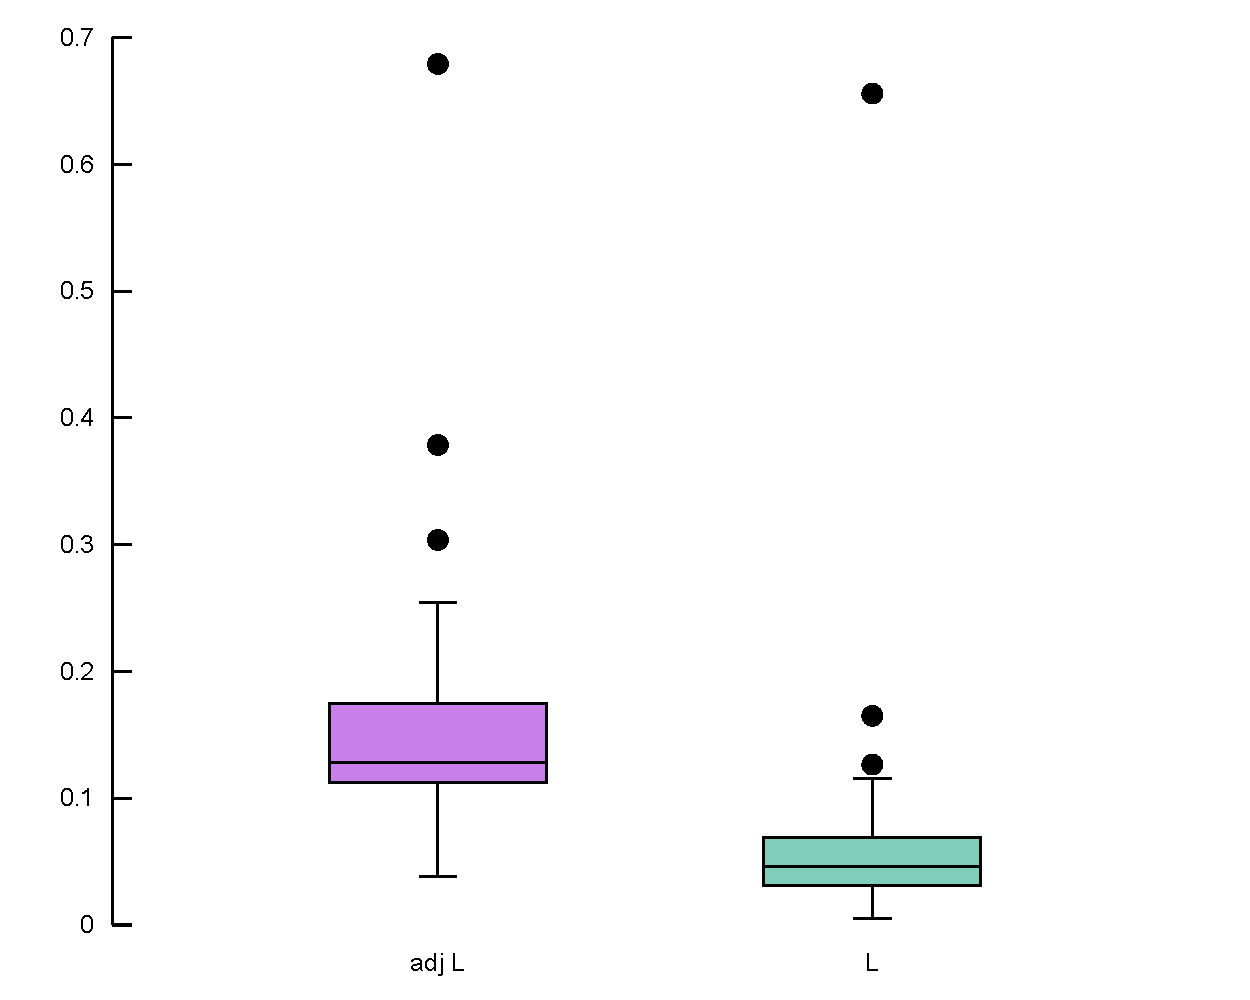
\includegraphics[width=0.9\linewidth]{img/box-swda.pdf}
  \caption{Box plot for dialogue acts associated with laughter in SWDA. On the left: proportion of DAs having laughter in one of the adjacent utterances, on the right: proportion of DAs containing laughter. }
    \label{fig:box-swda}
\end{figure}

\begin{figure}
  \centering
  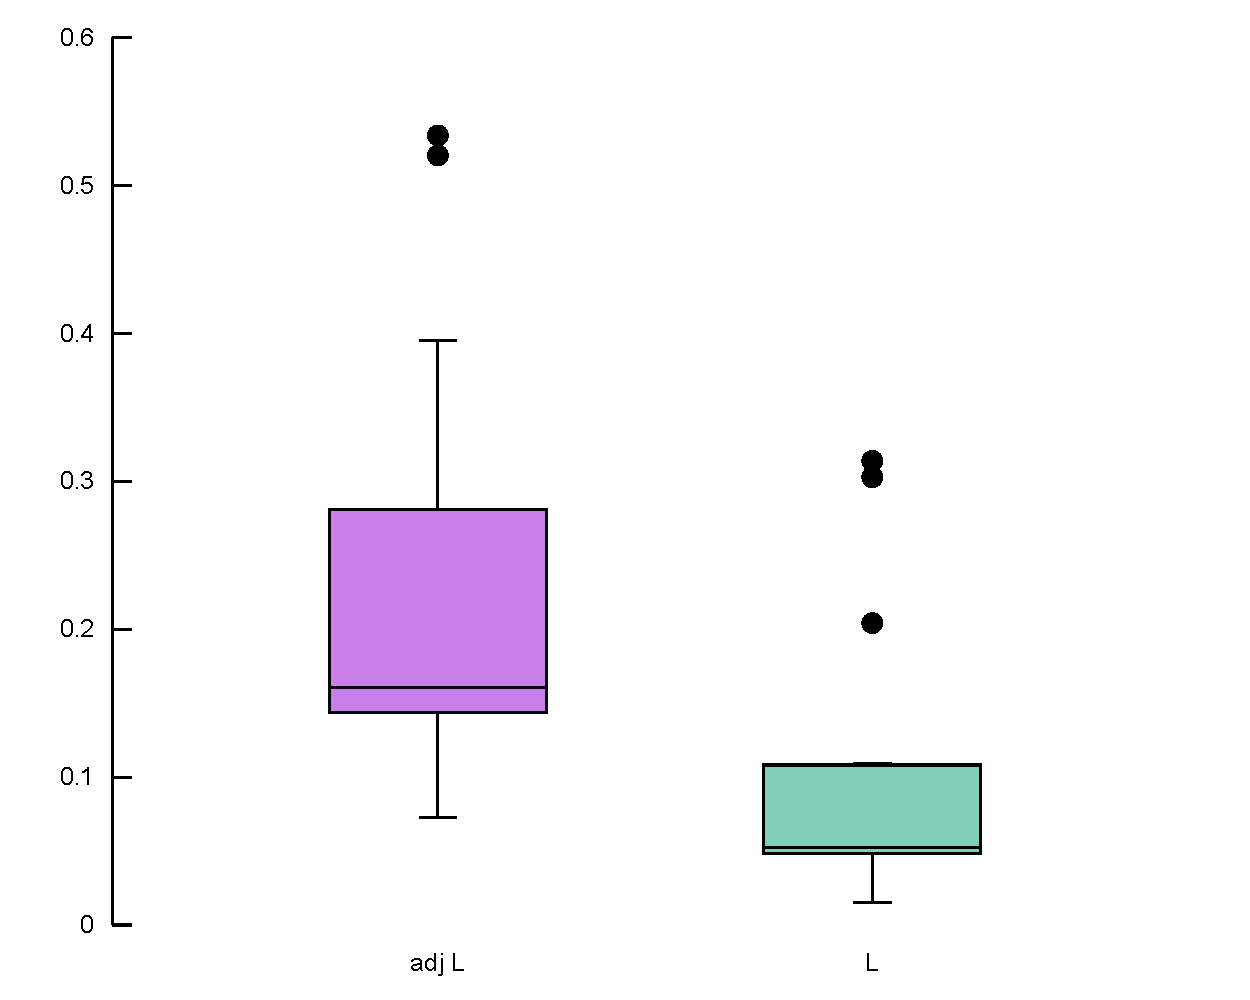
\includegraphics[width=0.9\linewidth]{img/box-ami.pdf}
  \caption{Box plot for dialogue acts associated with laughter in AMI-DA. On the left: proportion of DAs having laughter in one of the adjacent utterances, on the right: proportion of DAs containing laughter. }
    \label{fig:box-ami}
\end{figure}

\paragraph{Dialogue act grouping}
For our corpora we also considered grouping the dialogue acts according to DAMSL coders manual \citep{jurafskySwitchboardSWBDDAMSLShallowDiscourseFunction1997a}: Forward-Communicative-Function (51.86\% of all DAs), Backwards-Communicative-Function (30.35\%), Other (9.04\%) and Communicative-Status (8.75\%).
This allows the direct comparison between SWDA and AMI-DA.
With respect to laughs, we observed an even distribution of them in the groups, except for the Communicative-Status group in the case of SWDA, because of the ``Nonverbal'' dialogue acts (see footnote~1).
% - Preprocessing: remove disfluencies, acronyms and speaker tokens in AMI, removing laughter % Bill
  
\section{Model} % Bill

To test the effectiveness of BERT for DAR, we employ a simple neural architecture with two components: an encoder that vectorizes utterances, and a sequence model that predicts dialogue act tags from the vectorized utterances (Figure~\ref{fig:model-architecture}).
Since we are primarily interested in comparing different utterance encoders, we use a basic RNN as the sequence model in every configuration. 
The RNN takes the encoded utterance as input at each time step,
and its hidden state is passed to a simple linear classification layer over dialogue act tags.
Conceptually, the encoded utterance represents the context-agnostic semantic content of the utterance, and the hidden state of the RNN represents the full discourse context.

\begin{figure*}
  
\tikzstyle{rnn}=[rectangle,
  thick,
  minimum height=0.5cm,
  minimum width=2cm,
  fill=cyan]
\tikzstyle{encoder}=[rectangle,
  thick,
  minimum height=0.5cm,
  minimum width=2cm,
  fill=yellow]

\centering
\begin{tikzpicture}[>=latex,text height=1.5ex,text depth=0.25ex]
  \matrix[row sep=0.5cm,column sep=0.5cm] {
  % First line: Output labels
  \node (Y_0) []{$\hat{Y}_0$};&
  \node (Y_1) []{$\hat{Y}_1$};&
  \node (dots1) [] {$\dots$};  &
  \node (Y_T) []{$\hat{Y}_T$};&
  \\ % Second line: RNNs
  \node (RNN_0) [rnn]{RNN};&
  \node (RNN_1) [rnn]{RNN};&
  \node (dots2) [] {$\dots$};  &
  \node (RNN_T) [rnn]{RNN};&
  \\ % Third line: Linear layers
  \node (Encoder_0) [encoder]{Encoder};&
  \node (Encoder_1) [encoder]{Encoder};&
  \node (dots3) [] {$\dots$};  &
  \node (Encoder_T) [encoder]{Encoder};&
  \\ % Fourth line: Linear layers
  \node (Input_0) []{\small $ \underbrace{s^0,w^0_{0},w^0_{1},...,w^0_{n_0}}_{\text{Utterance 1}}$};&
  \node (Input_1) []{\small $ \underbrace{s^1,w^1_{0},w^1_{1},...,w^1_{n_1}}_{\text{Utterance 2}}$};&
  \node (dots4) [] {$\dots$};  &
  \node (Input_T) []{\small $ \underbrace{s^T,w^T_{0},w^T_{1},...,w^T_{n_T}}_{\text{Utterance T}}$};&
  \\ };
  \path[->]
  (Input_0) edge[thick]  (Encoder_0)	
  (Input_1) edge[thick] (Encoder_1)	
  (Input_T) edge[thick] (Encoder_T)	

  (Encoder_0) edge[thick] node[right] {} (RNN_0)	
  (Encoder_1) edge[thick] node[right] {} (RNN_1)	
  (Encoder_T) edge[thick] node[right] {} (RNN_T)	

  (RNN_0) edge[thick] (Y_0)	
  (RNN_1) edge[thick] (Y_1)	
  (RNN_T) edge[thick] (Y_T)	

  (RNN_0) edge[thick] node[above] {$h_1$} (RNN_1)
  (RNN_1) edge[thick] node[above] {$h_2$} (dots2)
  (dots2) edge[thick] node[above] {$h_T$} (RNN_T)
  ;
\end{tikzpicture}

  \caption{Simple neural dialogue act recognition sequence model}
  \label{fig:model-architecture}
\end{figure*}

As a baseline utterance encoder, we use a word-level CNN with window sizes of 3, 4, and 5, each with 100 feature maps \citep{kimConvolutionalNeuralNetworks2014}. 
The model uses 100-dimensional word embeddings, which are initialized with pre-trained gloVe vectors \citep{penningtonGloveGlobalVectors2014}.

For the BERT utterance encoder, we use the BERT\textsubscript{BASE} model with hidden size of 768 and 12 transformer layers and self-attention heads \citep[][\S3.1]{devlinBERTPretrainingDeep2018}.
In our implementation, we use the un-cased model provided by \citet{wolfHuggingFaceTransformersStateoftheart2019}.

\section{Experiments}
\subsection{Experiment 1: Impact of laughter} \label{sec:experiment1}   % Vlad
In the first experiment we investigated whether laughter, as an example of a dialogue-specific signal, is a helpful feature for DAR.
Therefore, we train another version of each model: one containing laughs (\texttt{L}) and one with laughs left out (\texttt{NL}), and compare their performances in DAR task.
Table~\ref{table:laughter-total-acc} compares the results from applying the models with two different utterance encoders (\texttt{BERT}, \texttt{CNN}).
First of all, we can see that \texttt{BERT} utterance encoder outperforms \texttt{CNN} in all the cases.
From observing the effect of laughters, we can see differences in performance depending on the dialogue act, regardless how often laughter occurs in the current or adjacent utterances (see Figure~\ref{fig:by-da} in Appendix~\ref{sec:suppl}).
The strongest evidence for laughter as a helpful feature was found in SWDA for the \texttt{BERT} utterance encoder, where macro-F1 score increases by 7.89 percentage points.

\begin{table}
  \centering
  \begin{tabular}{@{}lcccc@{}}
    \toprule
                      & \multicolumn{2}{c}{SWDA} & \multicolumn{2}{c}{AMI-DA} \\ \midrule
                      & F1    & acc.  & F1    & acc.       \\ 
    \texttt{BERT-NL}  & 38.10 & 77.07 & 49.09 & 67.06       \\ 
    \texttt{BERT-L}   & 45.99 & 76.93 & 50.17 & 67.12       \\ \midrule
    \texttt{CNN-NL}   & 37.23 & 75.08 & 38.37 & 63.46        \\
    \texttt{CNN-L}    & 27.59 & 75.40 & 37.94 & 64.30        \\ \bottomrule
    
  \end{tabular}
  \caption{Comparison of macro-average F1 and micro-average accuracy depending on using laughter on the training phase. }
  \label{table:laughter-total-acc}
\end{table}

Confusion matrices (Figure~\ref{fig:swda-cm}) provide some food for thought. Most of the misclassifications fall into the majority classes, such as \emph{sd} (Statement-non-opinion), in the left edge of the matrix. However there are some important exceptions, such as \emph{rhetorical questions}, that are misclassified as other forms of questions due to their surface question-like form.
Importantly, laughter helpes to classify rhetorical questions correctly, this is because in a conversation it can be used as a device to cancel seriousness \citep{ginzburg2015understanding}, in this case, of a question.
Therefore questions, like the one we show in the example in Table~\ref{table:example-qh}, are easier to disambiguate with the help of laughter.
\begin{table}
      \small
  \centering
  \begin{tabularx}{\linewidth}{llL}
    \toprule
    Speaker & DA & Utterance \\ \midrule
        \multicolumn{3}{c}{\emph{(Talking about hobbies)}}\\
    B   & sd	&  Um, as far as spare time, they talked about, \\
    B	& \% & I don't, + I think, \\
    B	& qh & who has any spare time \texttt{<laughter>}? \\
    A	& x & \texttt{<laughter>}.\\
             \bottomrule
  \end{tabularx}
  \caption{Example from the SWDA corpus (sw3735). B's contribution \emph{qh} (Rhetorical question) is misinterpreted as \emph{qw} (Wh-question) by the BERT model without laughs in training data. }
  \label{table:example-qh}
\end{table}



  \begin{figure}
  \centering
  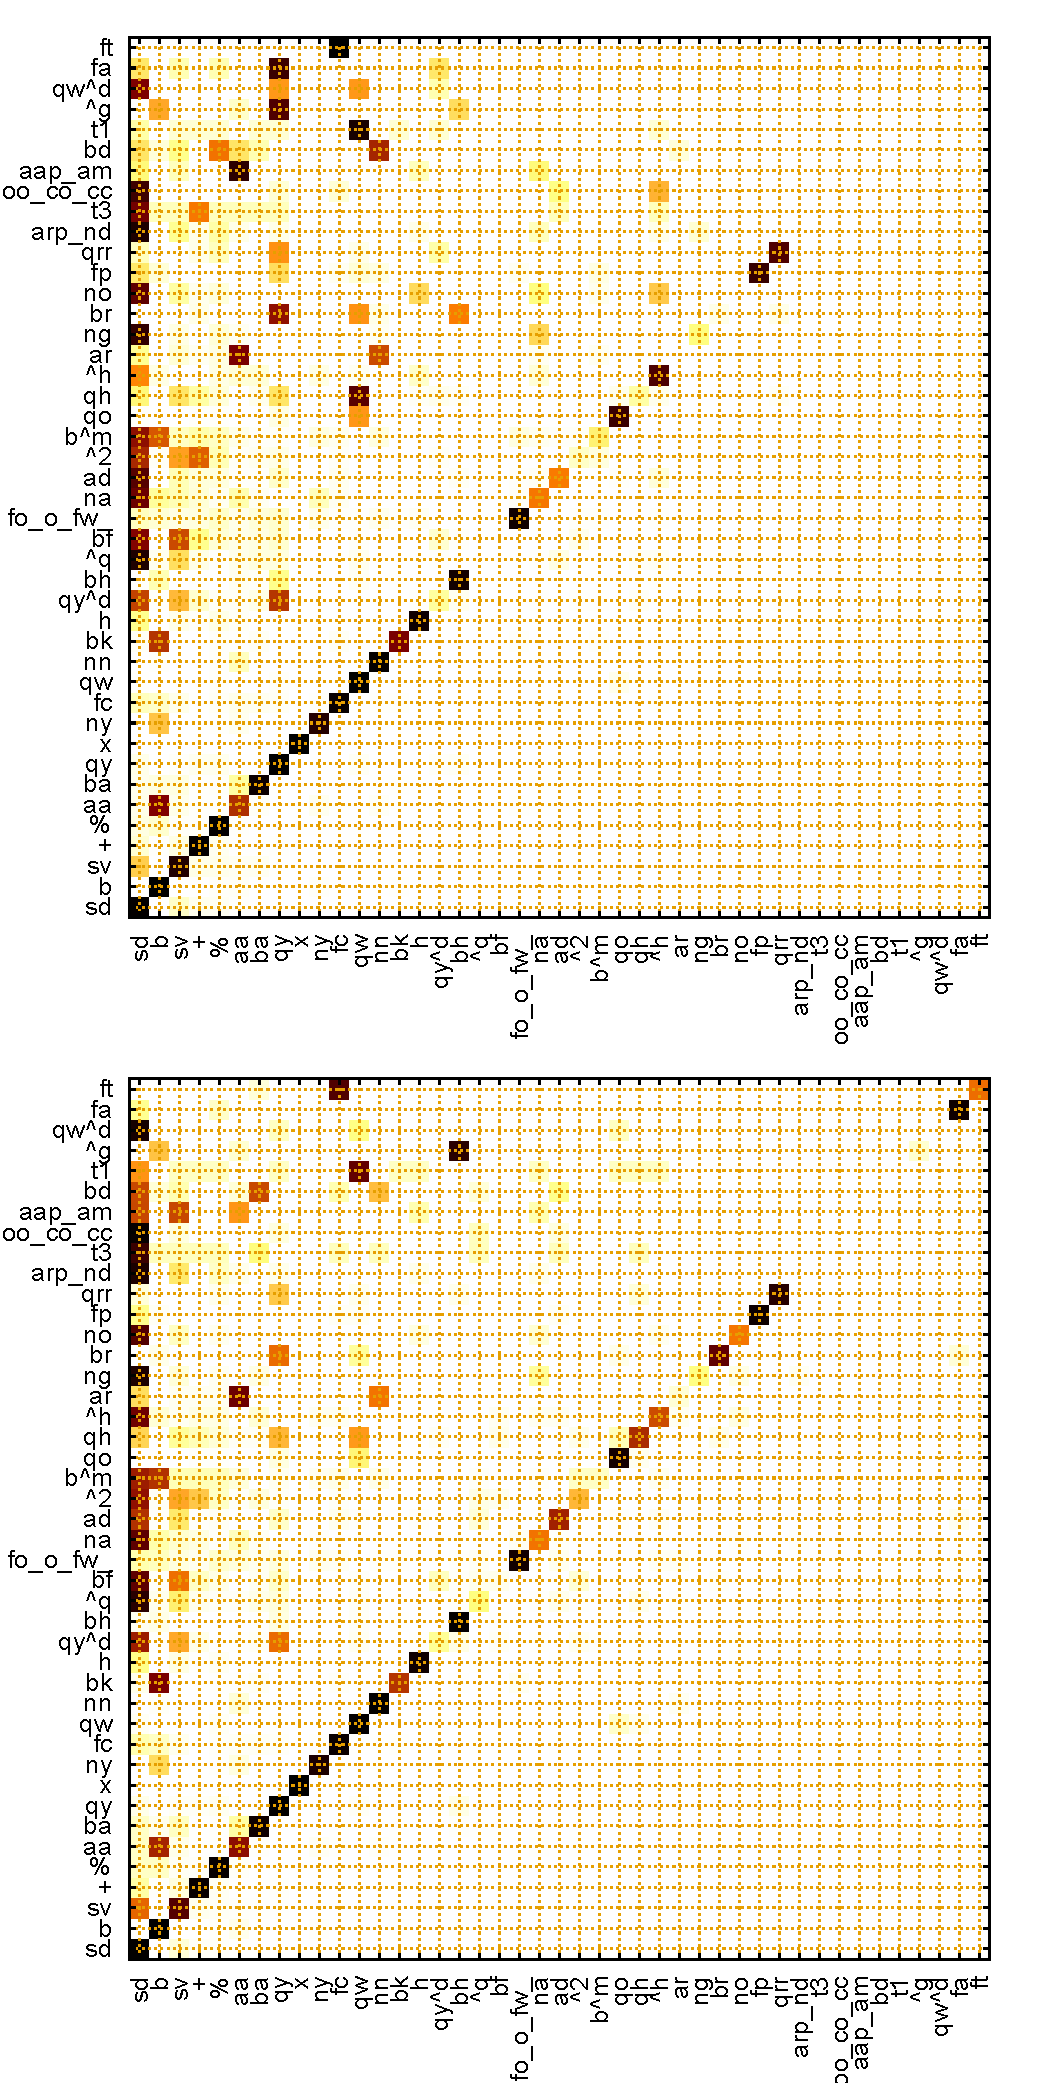
\includegraphics[width=1.0\linewidth]{img/swda-cm.pdf}
  \caption{Confusion matrices for \texttt{BERT-NL} (top) vs \texttt{BERT-L} (bottom); SWDA corpus. Solid line shows the improvement in classification of rhetorical questions.}
    \label{fig:swda-cm}
  \end{figure}

In order to further investigate the differences between the models and datasets, we looked at the dialogue act groups.
Mapping all dialogue acts into four groups allows direct comparison between model performances in SWDA and AMI-DA.
Table~\ref{table:laughter-group-acc} compares accuracies between the two main groups: Forward-Communicative-Function and Backward-Communicative-Function (82.3\% of all DAs in SWDA and 76.7\% in AMI-DA).
Our models tend to perform better for the Forward-Communicative-Function group for both corpora irrespective of the presence of laughs.
Also, our models perform better on the SWDA corpus.
Overall performance in these groups appears to be unaffected by presence of laughs.

\begin{table}
  \centering
  \begin{tabular}{@{}llcc@{}}
    \toprule
    &                  & Forw.-CF  & Backw.-CF   \\ \midrule
    \multirow{4}{*}{SWDA}    &\texttt{BERT-NL}  & 92.54 & 91.67       \\ 
                             &\texttt{BERT-L}   & 95.42 & 90.91       \\ 
                             &\texttt{CNN-NL}   & 93.30 & 90.85        \\
                             &\texttt{CNN-L}    & 94.64 & 90.13        \\ \midrule
    \multirow{4}{*}{AMI-DA}  &\texttt{BERT-NL}  & 87.77 & 80.83       \\ 
                             &\texttt{BERT-L}   & 87.36 & 79.87       \\
                             &\texttt{CNN-NL}   & 91.85 & 71.21        \\
                             &\texttt{CNN-L}    & 91.25 & 71.28        \\    \bottomrule
  \end{tabular}
  \caption{Comparison of models depending on using laughter on the training phase. }
  \label{table:laughter-group-acc}
\end{table}


\subsection{Experiment 2: Impact of pre-training vs. fine-tuning} \label{sec:experiment2} % Bill
Next, we analyze how pre-training affects BERT's performance as an utterance encoder.
To do so, we consider the performance of DAR models with three different utterance encoders:
\begin{itemize}
  \item \texttt{BERT-FT} -- pre-trained BERT with DAR fine-tuning 
  \item \texttt{BERT-RI} -- randomly initialized BERT (with DAR fine-tuning)
  \item \texttt{BERT-FZ} -- pre-trained BERT without fine-tuning (frozen during DAR training)
\end{itemize}

\begin{table}[]
\centering
\begin{tabular}{@{}lrrrr@{}}
\toprule
                           & \multicolumn{2}{c}{SWDA}                          & \multicolumn{2}{c}{AMI-DA}                        \\ \midrule
                           & \multicolumn{1}{c}{F1} & \multicolumn{1}{c}{acc.} & \multicolumn{1}{c}{F1} & \multicolumn{1}{c}{acc.} \\
\texttt{BERT-FT} & 45.99           & 76.93                    & 50.03                  & 66.94                    \\
\texttt{BERT-RI} & 32.18           & 73.80                    & 33.45                  & 61.53                    \\
\texttt{BERT-FZ} & 7.75            & 55.61                    & 14.44                  & 46.59 \\
  \bottomrule
\end{tabular}
  \caption{Macro-average F1 and micro-average accuracy of BERT with standard pre-training and DAR fine-tuning (\texttt{BERT-FT}) vs.~the same model without pre-training (\texttt{BERT-RI}) and without fine-tuning (\texttt{BERT-FZ}).}
  \label{table:exp2}
\end{table}

The pre-trained model is more accurate than the randomly initialized model by several percentage points on both DA corpora,
suggesting that BERT's extensive pre-training does provide some useful information for recoginizing different dialogue acts (Table~\ref{table:exp2}).
This performance boost is much more pronounced in the macro-averaged F1 score,
which is explained by the fact that at the tag level, pre-training has a larger impact on less frequent tags. 

A key aspiration of transfer learning is to expose the model to phenomena that are too infrequent to learn from labeled training data alone.
One explanation for pre-trained BERT's superior performance on some infrequent dialogue acts is that it has learned to represent relevant features
that the randomly initialized model was unable to learn due to their sparsity in the labeled training set.
Indeed, a simple lexical probe supports this explanation: in utterances where the pre-trained model is correct and the randomly initialized model is not,
the rarest word is 1.9 times rarer than is typical of corpus as a whole.

Comparing the performance of the fine-tuned encoder to that of the frozen model, we note that pre-training alone is not enough.
The frozen model is heavily biased towards the most frequent tags, which explains its especially poor macro-average score (Table~\ref{table:exp2}).
In SWDA, for example, the model with a frozen encoder predicts one of the two most common tags (Statement-non-opinion or Acknowledge) 86\% of the time, whereas those two
tags account for only 51\% of the ground truth tags.
The fine-tuned model is much less biased; it predicts the two most common tags only 59\% of the time.

%These observations raise two questions.
%First, how does BERT's pre-training help with DAR? 
%And second, in what way are the representations learned by pre-trained BERT lacking?
%In other words, what is the contribution of fine-tuning?

%To help answer these questions, we compare performance of the above three models by dialogue act tag.

% TODO: add per dialogue act accuracy figures

\paragraph{Fine-tuning and laughter}
Since the laughter token doesn't appear in the original BERT vocabulary, only fine-tuned models can meaningfully make use of laughter in utterance representations. 
This gives us another opportunity to assess whether laughter is useful in dialogue act recognition.
We find that although 4.6\% of utterances in SWDA contain laughter, 
7.3\% of utterances misclassified by the frozen model but correctly classified by the fine-tuned model contain laughter, 
suggesting that the fine-tuned encoder makes use of laughter. 
For AMI-DA, the effect is less pronounced, but still present: 
overall, 8.5\% of utterances contain laughter, 
compared to 9.6\% of utterances where fine-tuning makes a difference. 

\subsection{Experiment 3: Impact of dialogue pre-training} \label{sec:experiment3} % Bill

Next, we assess the effect of further in-domain pre-training on BERT's performance as an utterance encoder.\footnote{
In-domain pre-training is sometimes referred to as \textit{fine-tuning}, but we reserve that term for task-specific training on labeled data.}
We construct pre-training corpora from the SWDA portion of the un-labeled Switchboard corpus and from the entire AMI corpus (including the 32 dialogues with no human-annotated DA tags that are not included in the DAR training set).
In both cases, we exclude dialogues that are reserved for DAR testing.

We use the same pre-training task described by \citet{devlinBERTPretrainingDeep2018}, which combines masked token prediction and next sentence (utterance) detection. 
Distractor utterances are drawn at random from another dialogue in the corpus
and each epoch is generated separately so that different distractor sentences appear each time.
We pre-trained three BERT models: with Switchboard (10 epochs), AMI (10 epochs), and the combined corpus (5 epochs).

For each dialogue act corpus, we trained DAR models with BERT encoders pre-trained on the in-domain corpus (\texttt{BERT+ID}) and the combined corpus (\texttt{BERT+CC}).
As before, we experimented with both the fine-tuning and frozen conditions.

The results are mixed.
In-domain pre-training offers a modest boost in overall accuracy,
but the macro-average scores are almost uniformly worse (Table~\ref{table:exp3}).
%Indeed, when BERT is frozen during fine-tuning, the model that received no further pre-training performs better by more than 3 percentage points (Table~\ref{tab:exp3-recall}).
To fully assess the potential impact of further in-domain pre-training, a larger dialogue corpus is required.

% Please add the following required packages to your document preamble:
% \usepackage{booktabs}
\begin{table}[]
\begin{tabular}{@{}lrrrr@{}}
\toprule
           & \multicolumn{2}{c}{SWDA}                          & \multicolumn{2}{c}{AMI-DA}                        \\ \midrule
           & \multicolumn{1}{c}{F1} & \multicolumn{1}{c}{acc.} & \multicolumn{1}{c}{F1} & \multicolumn{1}{c}{acc.} \\
\texttt{BERT-FT}    & 45.99                  & 76.93                    & 50.03                  & 66.95                    \\
\texttt{BERT+ID-FT} & 45.48                  & 77.02                    & 46.56                  & 68.66                    \\
\texttt{BERT+CC-FT} & 47.78                  & 77.35                    & 48.72                  & 66.58                    \\ \midrule
\texttt{BERT-FZ}    & 7.75                   & 55.61                    & 14.44                  & 46.60                    \\
\texttt{BERT+ID-FZ} & 6.46                   & 52.30                    & 14.43                  & 48.07                    \\
\texttt{BERT+CC-FZ} & 5.76                   & 51.14                    & 12.56                  & 42.42                    \\ \bottomrule
\end{tabular}
  \caption{Comparison of macro-average F1 and micro-average accuracy  with further in-domain (\texttt{ID}) and cross-domain (\texttt{CC}) dialogue pre-training,
    for both the frozen (\texttt{FZ}) and fine-tuned (\texttt{FT}) conditions.}
  \label{table:exp3}
\end{table}


%\subsection{Experiment 4: Cross-domain pre-training (if time permits)} \label{sec:experiment4} % Bill
%  - cross-domain pre-training

\section{Discussion} % add items to discuss
On the question of laughter impact, this study found out that laughter is more helpful in SWDA corpus than in AMI-DA.
This observation may support the hypothesis that in SWDA due to the nature of interactions over the phone, dialogue participants can not rely on visual signals, such as gestures and facial expressions, therefore vocalisations, such as laughter, are more pronounced and therefore more helpful to disambiguate the utterances.

This also can explain why all our best models perform better on SWDA: much more information that interlocutors and dialogue act annotators can rely on is present in the transcription of SWDA, whereas AMI-DA annotators receive clear instructions to pay attention to the videos \citep{GuidelinesDialogueAct2005}.
This finding is consistent with that of \citet{bavelas2008gesturing} who demonstrated that in face-to-face dialogue visual components, such as gestures, can convey information that is independent from one conveyed with speech.


\begin{itemize}
  \item RoBERTa training scheme finds that next sentence prediction is of little importance. Is this true for us too? (suspect not due to discourse importance). see: https://github.com/huggingface/transformers/issues/1622
  \item Issues related to working with transcribed speech: Different kinds of laughter are all represented by the same token. Does transcription orthography capture prosody? We know prosidy is useful for DAR (Jurafsky).
  \item future work: pre-training on very large un-labeled dialogue corpora. How does text chat transfer to the spoken/transcribed setting?
  \item Laughter is more helpful in SWDA than in AMI-DA. 
  \item The point above can also explain why our models better on SWDA: just a larger proportion of stuff that interlocutors rely on is in the transcription.
\end{itemize}

\bibliography{acl2020}
\bibliographystyle{acl_natbib}
\clearpage
\appendix
\begin{figure*}[h!]
  \section{Supplementary materials}\label{sec:suppl}
  \centering
  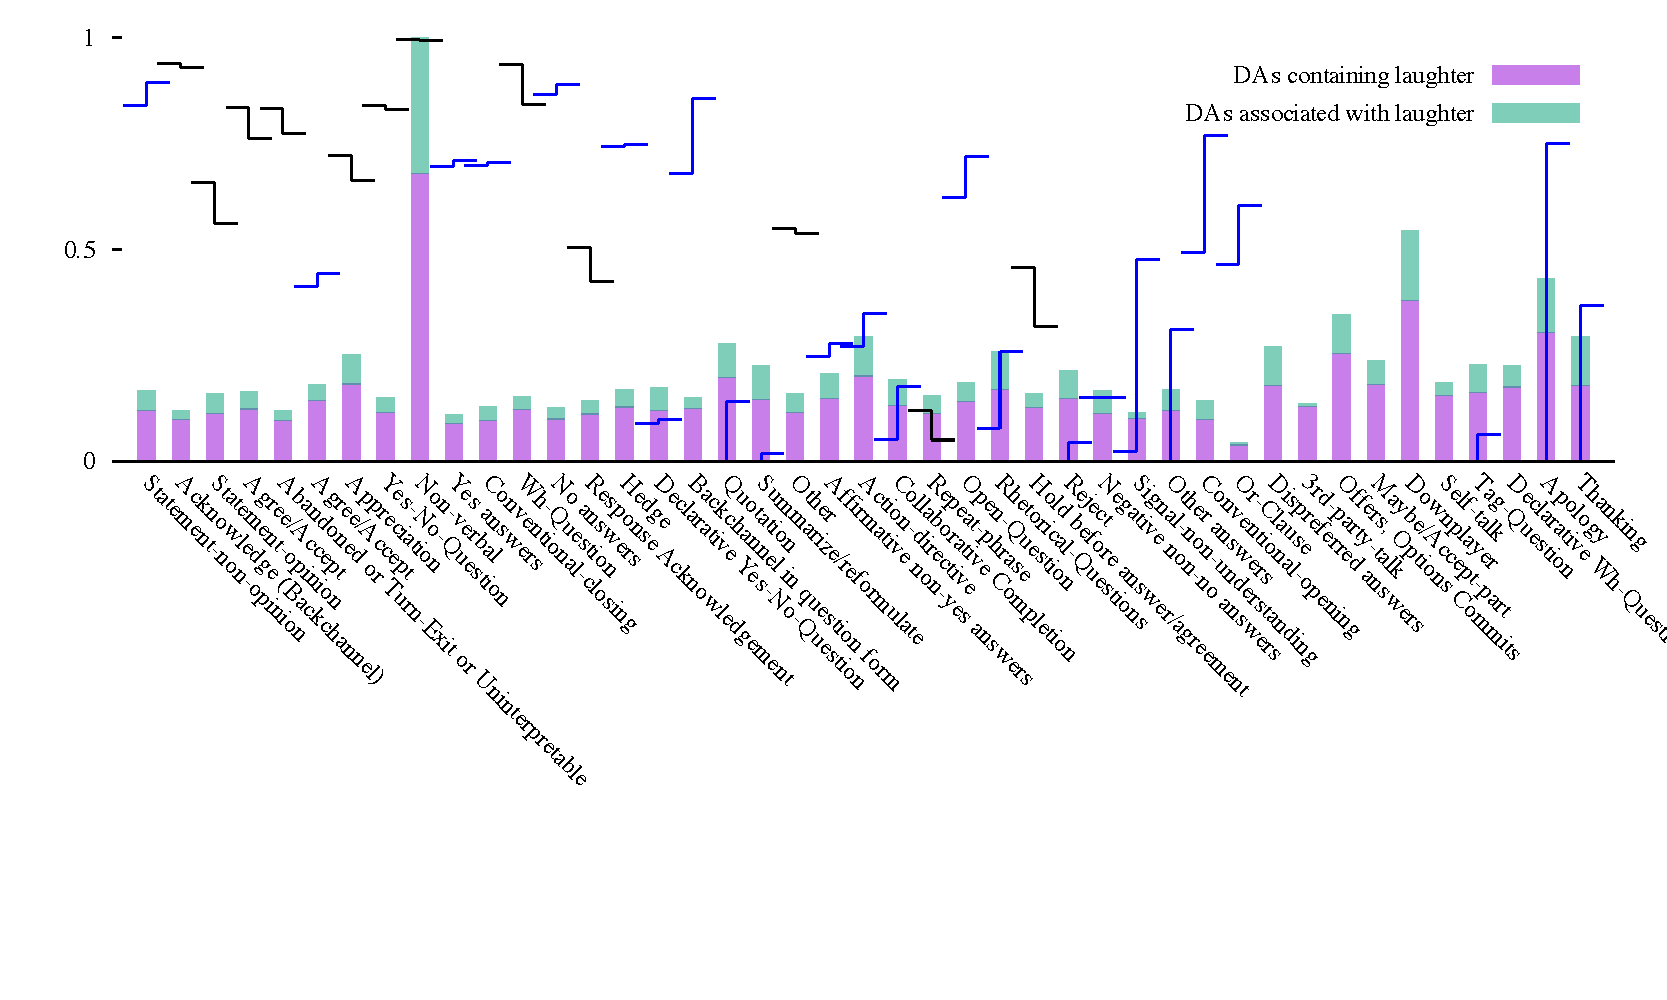
\includegraphics[width=\linewidth]{img/SWDA-bertLvsNL.pdf}
  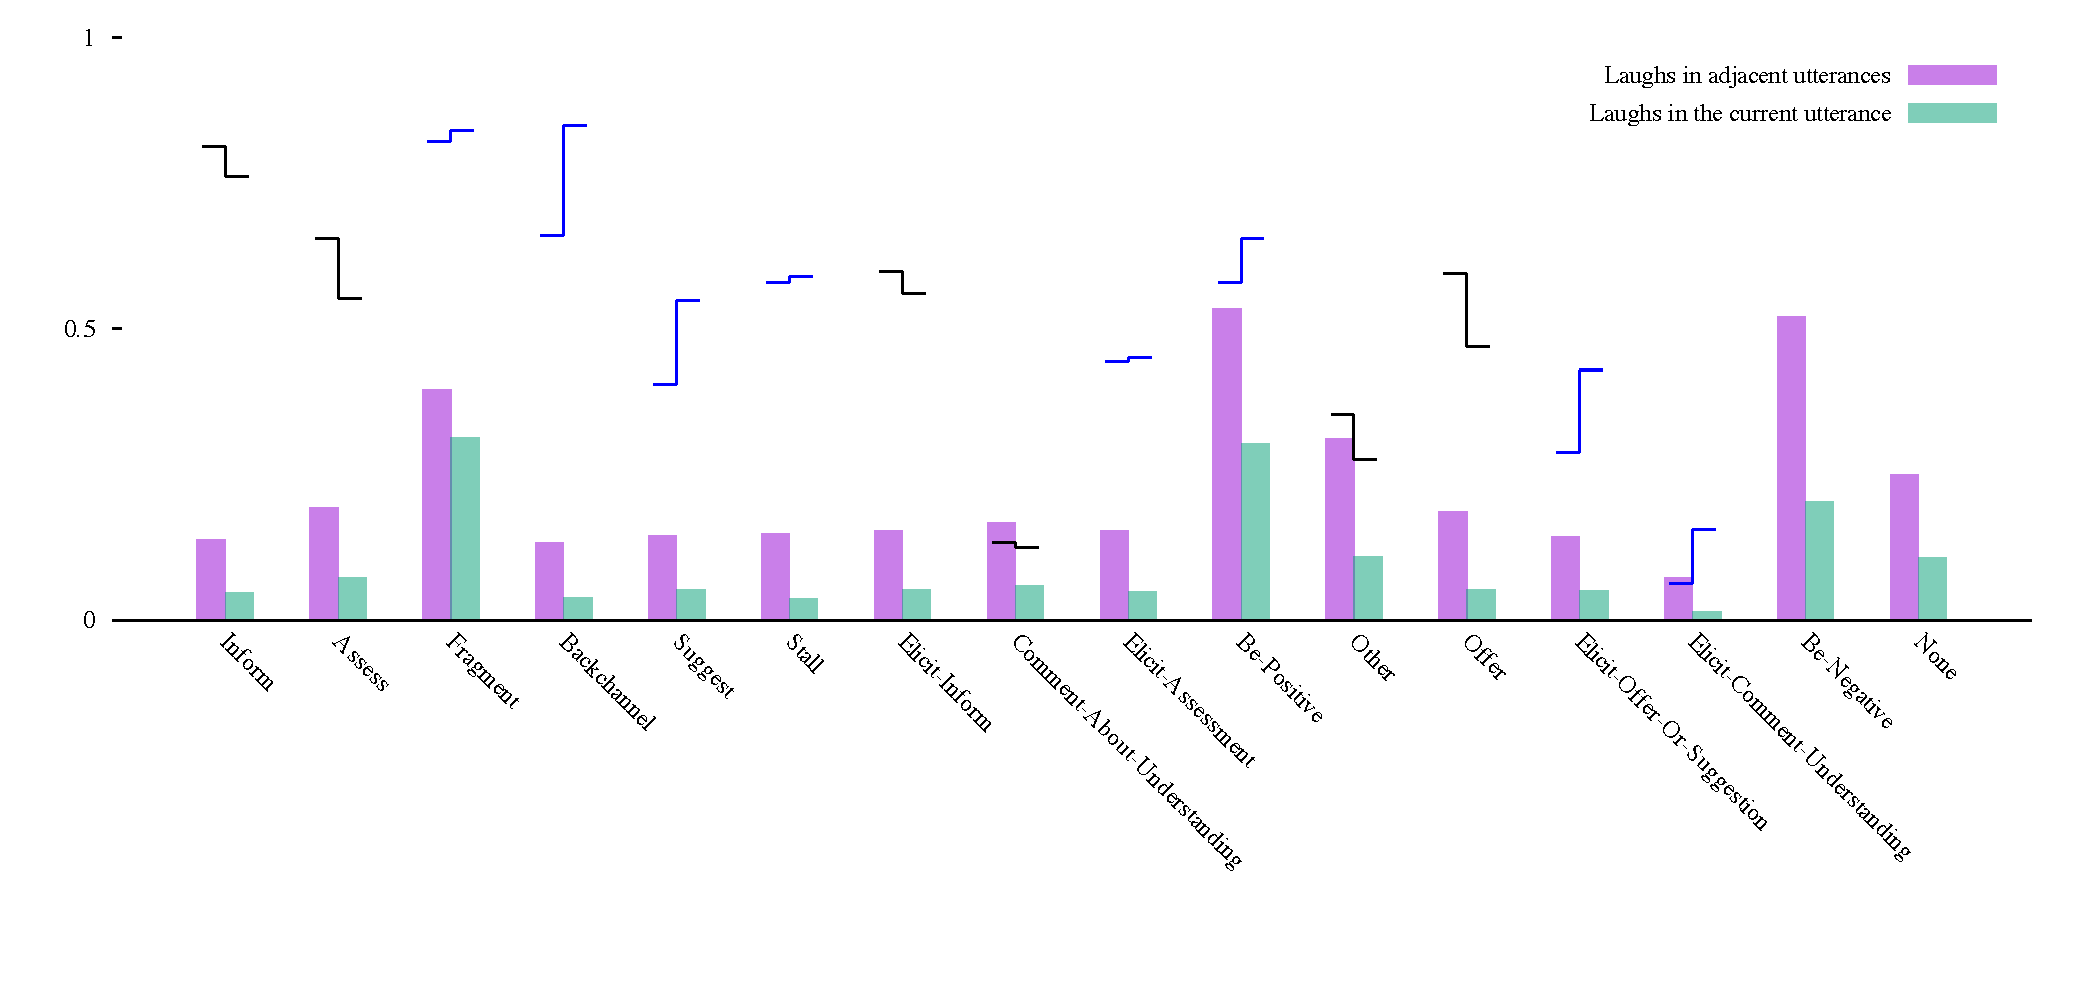
\includegraphics[width=\linewidth]{img/AMI-DA-bertLvsNL.pdf}
  \caption{Change in accuracy for each dialogue act (\texttt{BERT-NL} vs \texttt{BERT-L}). Positive changes when adding laughter (\texttt{BERT-L}) are shown in blue. Vertical bars indicate how often dialogue act is associated with laughter. Top chart: SWDA, Bottom chart: AMI-DA. }
    \label{fig:by-da}
  \end{figure*}



\end{document}
